% !TeX spellcheck = en_US
\chapter{State of the art}\label{chap: S-O-T-A}
This chapter presents the state-of-the-art approaches to various topics 
discussed 
in this article, including centralized and decentralized systems, 
\gls{mas}, \gls{dt}, network latency, 
and \gls{dsl} as a system modularization method. The article aims to 
design a program to fulfill the real-time communication requirements 
of specific use cases, in addition to analyzing and modularizing the 
timing behaviors. 
It builds on the works of leading researchers in the field.


\section{Centralized and decentralized systems}
Studies around centralized and decentralized systems have been conducted 
in many fields. It seems that globalization has gradually transferred the 
centralized top-down to decentralized bottom-up synthesis\cite{ueda_emergent_2004}.   
In the supply chain, for example, there is no longer a standalone production. Instead, 
a synergy of all vendors, customers, third-party providers, or other
firms\cite{mahapatra_modeling_2003}. This concept is carried over to be applied to multi-agent architecture. A comparison between centralized and decentralized 
architecture has been presented by service restoration with bus tests\cite{sharma_comparative_2016}. The 
analysis exposes the time taken by other system considerations, the impact 
of communication failure, and the impact of multiple fault scenarios, indicating 
that the decentralized system benefits from a lower computation time and cycles, 
not prone to single point failures, and efficient restoration of 
multiple faults. 
In \cite{egger_deployment-friendly_2020}, simulation and production tests 
for decentralized scheduling tasks have been conducted. In this paper, as shown 
in fig.\ref{fig: CentralizeDecentralizeConcept}, centralized and decentralized 
schemes are compared. In the centralized model, the master agent has the most power, 
while other agents serve as slaves without the ability to make their own decisions. 
However, in a \gls{mas}-based decentralized model, the production agents are 
capable of making decisions and interacting with each other under the coordination 
of the central customer interface agent. 

\begin{figure}[htb]
    \centering
    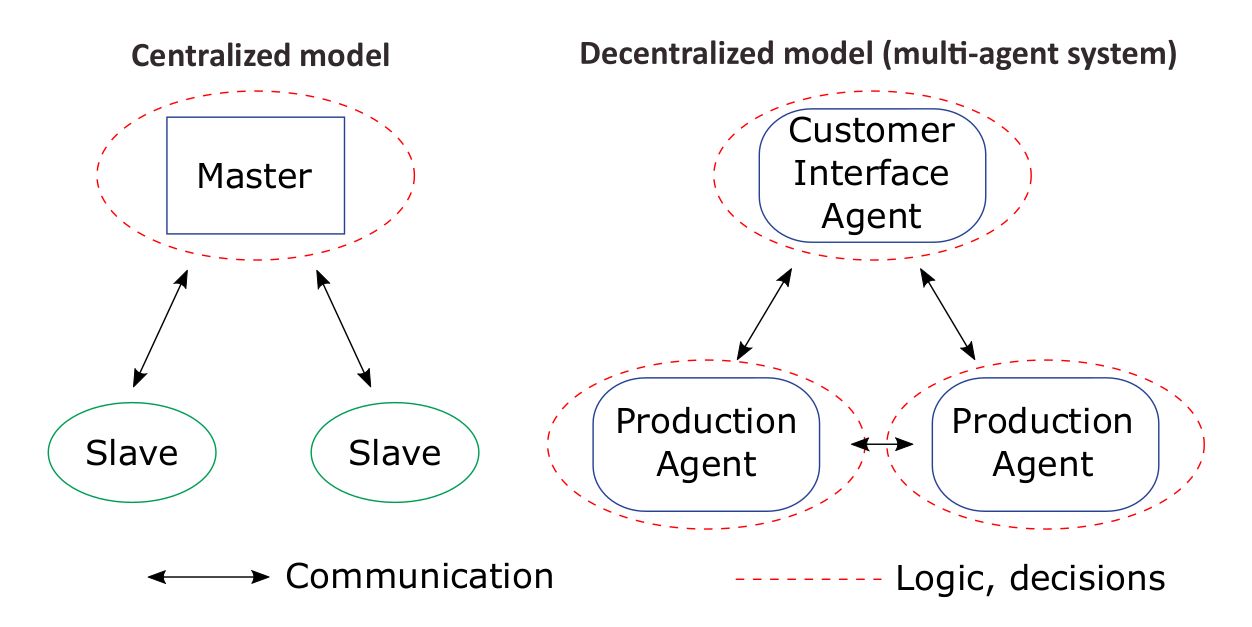
\includegraphics[width=0.8\textwidth]{figures/State-of-the-art/CentralizeDecentralizeConcept.png}

    \caption{Centralized vs. decentralized control schemes compared. 
    In the centralized model, decisions are made only within the 
    master, whereas in the decentralized model, decisions are taken 
    within local resources dependent on both local events or measurements 
    and information exchange with other resources. 
    Source: \cite[fig.1]{egger_deployment-friendly_2020}\label{fig: CentralizeDecentralizeConcept}}
\end{figure}



\section{MAS}

Within the subfields of \gls{mas}, an agent can be identified as a 
software agent with no physical embodiment but only software to control 
physical assets for different purposes. \textit{"In agent-oriented software 
development, an agent is a delineable software unit with a defined goal. 
An agent tries to achieve this goal through autonomous behavior, 
continuously interacting with its environment and other agents"}\cite{wagner_agentenunterstutztes_2008}. 
However, although not under discussion in this thesis, another 
interpretation of \gls{mas} can be a Multi-agent robot system that 
each agent represents an actual physical object, such as an individual 
robot that participates in the complex task execution\cite{ota_multi-agent_2006}.   


Defining \gls{mas} can be confusing, as different researchers approach 
it from various aspects. For a more unambiguous interpretation of the 
concept, a general \gls{mas} can be divided into three views: the 
technical system that comprises robots, the automation control system 
characterized by sensors, actuators, networks, and robot control units, 
and the technical process that describes the production process of the 
product\cite{lauber_prozessautomatisierung_1999}\cite{wannagat_agent_nodate}. 
The focus of this thesis is mainly on the technical system, which can 
be interpreted as a union of robots in a smart factory, with less 
emphasis on the components or functions executed by each robot for 
a specific movement.

For further discretization of an agent, whether the agent is product, 
process, or resource-oriented, an appropriate agent architecture should 
be chosen according to different considerations. There are several of 
them that should be emphasized: \gls{ra}, \gls{ca}, and \gls{ams}. 
\gls{ra} is an agent at the field level representing a single robot. 
Different from the other agents, \gls{ra} should be able to combine 
the modules with physical entities by choosing an appropriate design 
pattern. Therefore, comparing design patterns in different production 
levels is done\cite{ocker_leveraging_2021}. The choice of an ideal 
design pattern should be limited for \gls{ra} in this research by 
comparing three relevant design patterns:  \gls{ra} pattern in Wannagat’s 
architecture, \gls{mfs} patterns in Fischer’s architecture and 
self*-control 
MAS in Ryashentseva’s architecture. Among all,  Wannagat’s architecture\cite{cruz_salazar_cyber-physical_2019} 
is chosen as the appropriate design pattern for \gls{ra} for field level 
control, which consists of five modules: Planning Module, Knowledge Base, 
Control Module, Diagnosis Module, and communication interface. 
All modules are interconnected, meanwhile, with each bound to 
I/Os of a physical system and a communication interface to interact 
with other \gls{ras} or \gls{ams} through \gls{ca} \cite{cruz_salazar_cyber-physical_2019}. 
\gls{ams} and \gls{ca} should have different specifications in the 
same design pattern. \gls{ca}, for example, should be able to coordinate 
the message-based communication between the agents as a "mailbox" 
between them. In contrast, \gls{ams} plays an important role in the 
centralization and coordination of all other agents \cite{wannagat_entwicklung_2010}. 
\begin{figure}[htb]
    \centering
    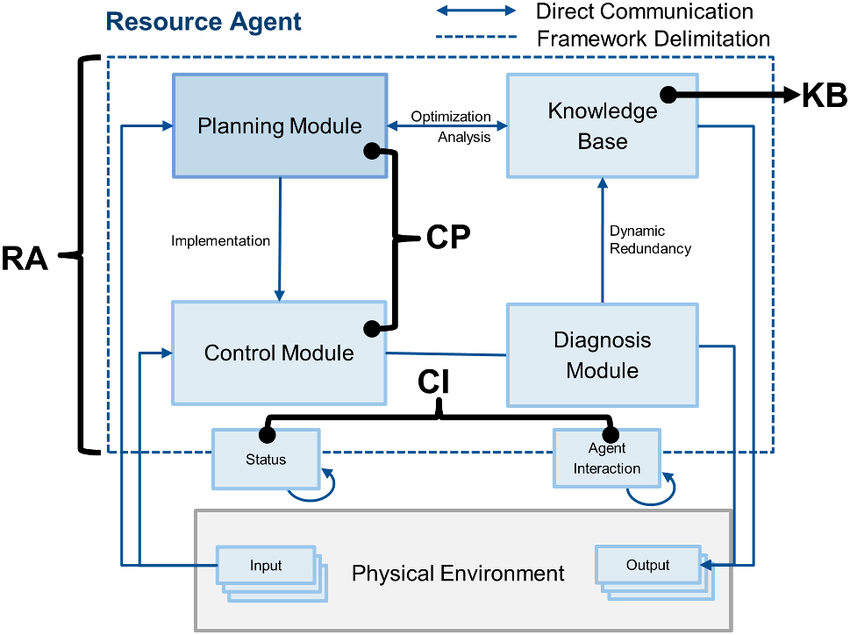
\includegraphics[width=0.8\textwidth]{figures/State-of-the-art/Wannagats-RA-pattern.png}

    \caption{Wannagat's \gls{ra} architecture.
    Source: \cite[fig.1]{cruz_salazar_cyber-physical_2019}\label{fig: Wannagat RA}}
\end{figure}



\section{Network communication}
According to early studies on network delays, the \gls{rtt} and \gls{owd} 
can either be measured by end-to-end methods or estimated with modeling 
approaches. Experiments have led to the consideration that \gls{tcp}-based 
measurements offer a practical solution for evaluating the movement of 
packets from end to end, along with a high packet retransmission rate 
to avoid packet loss\cite{paxson_end--end_1999}. Benefits from 
the development of the internet latency test tools, \gls{tcp} delay 
performance can be evaluated by one of them. Wireshark, for example, is famous 
for capturing network delay in the transport layer, where \gls{tcp} delay 
can be filtered in real-time\cite{dsouza_transmission_2020}. Besides, 
application and presentation layer delays can also be measured by Wireshark and 
other program-specific profiling tools\cite{heger_application_2017}. Furthermore, 
traceroute or ping can be utilized 
for network layer delay collections along with the router logs\cite{Deri2003}. 
Finally, it will be challenging to measure 
data link and physical layer delays, which can be either tracked by hardware 
such as \gls{nic} or calculated based on the characteristics 
of the physical medium. The work of \cite{Fezeu2023}, for example, 
presents a comprehensive, 
in-depth measurement study of mmWave 5G latency performance on the physical layer 
based on a commercial 5G tool.   
Certainly, there are also other tools designed for research for a more 
precise and academic-oriented purpose. In the work of performance testing 
of a 5G campus network, \gls{ftt} designed by ifak Magdeburg was used 
for performance analysis of industrial communication networks\cite{cainelli_performance_2023}, 
with its results later compared with those in this article.


On top of the measured delay 
that includes additional connection establishment and process time, 
models can be built additionally to estimate delays over different layers in 
\gls{osi} model to bridge the gap between experiments and simulations. 
Meanwhile, \gls{tcp/ip} model\cite{cerf1980protocols} is 
used more often in practical implementation 
for its simplicity, real-world alignment, while \gls{osi} model serves a more theoretical 
and sometimes too detailed for network modeling purposes. 
Studies including those for instance the modeling of \gls{tcp}-based 
packet transmission latency that enables both short and 
long \gls{tcp} flows\cite{luan_estimating_2019}. In the book \cite{wehrle2010modeling}, 
both lower and higher-layer wireless modeling tools and methods are introduced. 
Accordingly, common tools and methods for network simulation are ns-3 Network Simulator, OMNeT++, 
IKR Simulation Library and Open WNS. For the lower layer modeling, accurate simulation 
of physical layers can be operated, with the packet domain physical layer simulation 
model given as an example. Another lower-layer modeling approach should be focused on 
link layers, including \gls{mac} and logical link control. As for the higher layer 
modeling, modeling of the network layer and routing protocols, modeling 
transport layer protocols, and the modeling of application traffic are described. 
The combination of lower and higher layers results in the discrete modeling 
of the \gls{osi} model, with their performances tested in different use cases. 




By comparing both estimated and measured delays, a number of insightful 
conclusions made and the corresponding actions can be taken to improve 
the network design.
In the related work for delay measurement of \gls{mas}, 
a comparison between actual and modeling 
delays has been performed\cite{vogel-heuser_delay_2023}, which leads to the 
consideration of integrating \gls{dsl} as further development methods.





\section{\gls{dsl}}
To analyze and optimize the network communication performance, a deeper 
inspection of the network latency is needed. \gls{dsl} has, so far, reached 
some improvements in simplifying the design, presentation, and execution of 
network performance testing for many applications, including server-client applications 
based on hand-coded C, which minimizes the overhead produced by the compiler by 
comparing C and the designed \gls{dsl} based toolset under worst-case scenarios.
A level higher will be the agent-based \gls{dsl} that also includes network-based 
agent communication. The consideration of designing a \gls{dsl} framework 
for the agent's development has been discussed\cite{judith_domain_2013}. Another 
research for fulfilling real-time requirements for safety-critical and 
security-critical engineering has also adapted the \gls{dsl}, which aims to 
modularize the whole \gls{iot} system into a four-level architecture\cite{sklyar_domain_2022}. 



Another notable field for \gls{dsl} is the robotics. Unlike being widely 
used in industrial automation for modeling hard real-time constraints with 
a set of symbols that capture delays from networks and devices, I/O interfaces, 
and industrial controllers\cite{hujo_toward_2022}, \gls{dsl} for robotics is still 
under development due to its higher level of complexity and flexibility in 
robot control. Most of the time, a network communication system is integrated into a group 
of robot operations. To bridge the gap between the highly modularized automation system 
and robotic system, \gls{dsl4ras} for the software and hardware 
properties of robotic drive components are to be defined to meet the need 
of developing a robot-like system based on \gls{dsl}. In the recent work\cite{vogel-heuser_delay_2023}, 
the adaptation of \gls{dsl} is even more straightforward by adopting and 
extending the graphical notations 
from \cite{hujo_toward_2022} and \cite{volpert_supporting_nodate}. It, however, 
leaves the space for further extension. 



The starting point of a requirements-specific \gls{dsl} design is usually 
the existing software. 
A large amount of \gls{dsl} based visualization tools are mostly developed 
to be applied to an open-source robotics middleware suite such as \gls{ros}. 
For example, \gls{rviz} is a \gls{dsl} based 3D 
visualization tool for \gls{ros} that can visualize the robot model and 
capture sensor/actuator information. Movelt, also designed for \gls{ros}, 
provides a set of visual notations that represent the robot kinematics, 
motion planning, and many more. It also allows users to capture the 
timing behaviors of the bounding I/Os. Other middleware tools have been 
developed, but most are hardware and software-dependent. RobotML, a 
Robotic Modeling Language is designed for cross-platform robotic 
software development\cite{hutchison_robotml_2012}. It is developed 
based on Port and Connector to
capture the concept of an interaction between robot systems, including 
Robot, SensorSystem, ActuatorSystem, and LocalizationSystem, with its toolchain 
provided\cite[fig.5]{hutchison_robotml_2012}.



\section{\gls{dt}}


As mentioned earlier in chapter \ref{chap: Motivation}, 
\gls{dt} is a digital mapping of physical entities. Being a rather new concept to 
industrial automation systems, \gls{dt} has gained a lot of attention as a key concept 
of Industry 4.0. According to the existing research on \gls{dt}, their 
directions can be roughly divided into the following categories. The first one 
focuses on the real-time monitoring and visualization of physical assets or systems. 
A \gls{dt} visualization architecture for \gls{fms} has been designed to present 
the high-value information for lifecycle planning, design, debugging, and service 
stages by\cite{fan_digital-twin_2021}. In some cases, the visualization of \gls{dt} 
can be presented in a way for \gls{hmi}\cite{schroeder_visualising_2016}. 


The next orientation of \gls{dt} includes data analytics to support 
learning and decision-making. In a case study of wind power, the data from 
a \gls{dt} model is taken to feed both the physics-based and 
machine learning models\cite{erikstad_merging_nodate}. The processed 
data will be then either stored in a \gls{db} or presented in a regression model. 
Another exemplary \gls{dt} design that has contributed rich functionalities to 
data analytics is the \gls{imt} \gls{dt}\cite{tong_real-time_2020}. 
It contains a data analysis module 
that includes algorithms for error estimation, trajectory kinematics/dynamics 
transformation, machining vibration modal analysis, and a cutting force
estimation.

Based on the data analysis model, predictions can be made to handle failures and 
optimize resources. In \cite{katalinic_digital_2018}, known models are used to solve static and dynamic 
diagnostics tasks and the application for technical process optimization. To fill the 
gaps in maintainence prediction utilizing \gls{dt} big data analytics, a framework 
is designed to support the sharing of data, knowledge, and resources, with a 
mathematical programming model integrated\cite{mi_prediction_2021}. 


The last biggest challenge for \gls{dt} development will be the security threats. 
Although it benefits from breaking the edges in Industry 4.0, industrial stakeholders 
become more and more conservative. The threats exist but are not limited to the following 
fields: software attack, Privilege escalation, Man-in-the-middle, Rogue \gls{dt} 
servers and infrastructures and DT service tampering\cite{alcaraz_digital_2022}. Some possible solutions to these 
threats have been introduced, including the improvement of Identity, Authentication 
and Authorization, 
Hardware and Software Security, Hardening of DT Infrastructures and Decoupling, and many 
more. The gain of trust-worthy technologies to overcome security issues will certainly 
gain the confidence of potential \gls{dt} users. 



Our studies for the \gls{dt} part are based on the 
former work for this 
project, which has already provided a foundation for the \gls{dt} 
structure\cite{hofgen_architecture_2023}. 
The work mainly focuses on the realization of an \gls{aas} based Azure \gls{dt} system, 
with an automated \gls{dt} creation and socket-based communication between 
different layers from the \gls{dt} architecture reference 
model\cite[fig.5]{aheleroff_digital_2021}. In our work, the functionalities of \gls{dt} 
will be further investigated with an additional agent-based consideration. 


\section{Real-time requirements for collaborative robot systems}
Throughout our research, the real-time capability is an important metric for connecting 
various systems and components in \gls{cps}. However, it is not easy to define the 
real-time requirements, which vary greatly due to the system's complexity, 
system interaction requirements, hardware capability, and network latency, 
along with others. 
A use case based real-time requirements for low latency and high reliability 
is defined by\cite{li_5g_2018}, with the floor-level end-to-end latency 
approximately ranging from 1 to 10ms, and the remote control with about 50ms for a 5G 
system. However, according to\cite{zhang_infrastructure_2017}, the real-time 
\gls{qos} requirements for cloud applications (e.g.,\gls{ms} Azure and Amazon Web Service) 
could be selected by a real-time \gls{qos}-aware multicriteria decision-making 
technique. From the paper, an example is given in the gaming industry that has 
high real-time streaming requirements. Hence, the real-time requirement is not unique, and the decision-making for hard or 
soft real-time requirements should be executed in the design stage. 

\section{Research gap}

According to current research, there are various implementations of \gls{mas} in 
different fields. However, there have been limited efforts to standardize and 
modularize the \gls{mas} especially within the field of agent-based communication. 
In addition, a cloud-based resource digitization should also 
be considered and implemented in the \gls{mas}. In general, the \gls{mas} should be designed 
with a high level of modularization based on \gls{dsl}.

